\section{But du projet}
Le but de ce projet est d'implanter l’algorithme d’\emph{Aho-Corasick} pour compter le
nombre d’occurrences exactes d’un ensemble de \textit{k} mots dans un texte.
Nous devions utiliser trois méthodes pour représenter l’arbre :
\begin{itemize}
\item une matrice de transitions ;
\item un tableau de listes d’adjacence ;
\item une table de transitions pour la racine et un tableau de listes d’adja-
cence pour les autres noeuds de l’arbre.
\end{itemize}
Les exécutables devaient impérativement être nommés \textbf{ac-matrice},
\textbf{ac-liste}, \textbf{ac-mixte} respectivement et prendre deux paramètres,
d’abord le nom du fichier qui contient les mots à rechercher (un par ligne) puis
le nom du fichier qui contient le texte.

\section{Contenu de l'archive}
\dirtree{%
.1 bin \DTcomment{Contient les exécutables}.
.2 ac-liste \DTcomment{Aho-corasick avec des listes}.
.2 ac-matrice \DTcomment{Aho-corasick avec des matrices}.
.2 ac-mixte \DTcomment{Aho-corasick mixte}.
.2 genere-mots \DTcomment{Générateur de mots}.
.2 genere-texte \DTcomment{Générateur de texte}.
.1 gen \DTcomment{Contient les mots et textes générés}.
.1 obj \DTcomment{Objets issus de la compilation}.
.1 scripts \DTcomment{Scripts de démonstration}.
.2 clean.sh \DTcomment{Nettoie le projet et les fichiers générés}.
.2 run.sh \DTcomment{Script de démonstration du projet}.
.1 src \DTcomment{Sources du projet}.
.2 include \DTcomment{En-têtes des sources}.
.1 log.csv \DTcomment{Contient un rapport sur les temps d'éxécution}.
.1 makefile \DTcomment{Makefile du projet}.
.1 rapport.pdf \DTcomment{Ce rapport}.
.1 README.txt \DTcomment{Utilisation rapide du projet}.
}

\newpage
\section{Utilisation des programmes}
Les commandes ci-dessous se font depuis le dossier racine du projet décompréssé.

\subsection{Script de démonstration}
Le programme de démonstration construit le projet, génère pseudo-aléatoirement des
textes de longueur 5 000 000 sur des alphabets de taille 2, 4, 20 et 70, puis
pour chacun des alphabets génère pseudo-aléatoirement 3 ensembles de 100 mots de
longueur entre 5 et 15, entre 15 et 30 et entre 30 et 60 respectivement.
Ensuite, il exécute pour les 3 types de trie la rechereche des 3 ensembles dans
les textes respectifs, ce qui fait en tout 36 exécutions. Ces programmes
remplissent un fichier log.csv permettant de comparer les résultats.

La commande est la suivante :
\begin{minted}[gobble=4,framesep=5mm]{sh}
    ./scripts/run.sh
\end{minted}

\subsection{Programme de génération de mots}
Le programme affiche sur la sortie standard une série de mots séparés par un
retour chariot, que l'on peut rediriger dans un fichier.

La commande est la suivante :
\begin{minted}[gobble=4,framesep=5mm]{sh}
    ./bin/genere-mots NOMBRE MIN_SIZE MAX_SIZE ALPHA_SIZE
\end{minted}

Les paramètres sont les suivants :
\begin{itemize}
\item \textbf{NOMBRE} : le nombre de mots à obtenir ;
\item \textbf{MIN\_SIZE} : la taille minimale d'un mot ;
\item \textbf{MAX\_SIZE} : la taille maximale d'un mot ;
\item \textbf{ALPHA\_SIZE} : la taille de l'alphabet utilisé.
\end{itemize}

\subsection{Programme de génération de texte}
Le programme affiche sur la sortie standard le texte obtenu, que l'on peut
rediriger dans un fichier.

La commande est la suivante :
\begin{minted}[gobble=4,framesep=5mm]{sh}
    ./bin/genere-texte LENGTH ALPHA_SIZE
\end{minted}

Les paramètres sont les suivants :
\begin{itemize}
\item \textbf{LENGTH} : la taille du texte à obtenir,
\item \textbf{ALPHA\_SIZE} : la taille de l'alphabet utilisé.
\end{itemize}

\subsection{Comptage du nombre d'occurences d'un ensemble de mots dans un texte}
Pour les trois programmes suivants, \textbf{MOTS} est le fichier contenant l'ensemble de mots
séparés par un espace, \textbf{TEXTE} est le fichier comprenant le texte à rechercher,
et \textbf{LOGFILE} est un paramètre optionnel permettant de changer le fichier des résultats
(par défaut log.csv). Si ce fichier n'existe pas, il est créé, sinon, les résultats
sont ajoutés à la suite des précédents.

\subsubsection*{Avec une matrice de transisitions}
La commande est la suivante :
\begin{minted}[gobble=4,framesep=5mm]{sh}
    ./bin/ac-matrice MOTS TEXTE [LOGFILE]
\end{minted}

\subsubsection*{Avec un tableau de listes d'adjacence}
La commande est la suivante :
\begin{minted}[gobble=4,framesep=5mm]{sh}
    ./bin/ac-liste MOTS TEXTE [LOGFILE]
\end{minted}

\subsubsection*{En mixte}
La commande est la suivante :
\begin{minted}[gobble=4,framesep=5mm]{sh}
    ./bin/ac-mixte MOTS TEXTE [LOGFILE]
\end{minted}

\newpage
\section{Structures de données}
\subsection{Liste ordonnée}
Cette liste ordonnée contient un caractère (le caractère du noeud), l'identifiant
du prochain noeud ainsi que l'élément suivant. Elle est triée par ordre alphabétique, car cela permet de
récupérer plus rapidement une suite de lettres avec l'itérateur intégré.

\begin{minted}[mathescape,linenos,numbersep=5pt,gobble=4,frame=lines,framesep=5mm]{c}
    typedef struct _listelem *ListElem;

    struct _list {
        ListElem hd;
        ListElem it;
        size_t len;
    };

    struct _listelem {
        unsigned char c;
        size_t id;
        ListElem nx;
    };

    typedef struct _list *SortedList;
\end{minted}
\begin{center}\textit{Structure d'une liste ordonnée.}\end{center}

\subsection{Trie matriciel}
\begin{minted}[mathescape,linenos,numbersep=5pt,gobble=4,frame=lines,framesep=5mm]{c}
    struct _trie {
        size_t max;
        size_t next;
        size_t **trans;
        unsigned *finite;
        bool *truefinite;
        size_t *fallback;
    };
\end{minted}
\begin{center}\textit{Structure d'un trie matriciel.}\end{center}

\newpage
\subsection{Trie en liste}
\begin{minted}[mathescape,linenos,numbersep=5pt,gobble=4,frame=lines,framesep=5mm]{c}
    struct _trie {
        size_t max;
        size_t next;
        SortedList *trans;
        unsigned *finite;
        bool *truefinite;
        size_t *fallback;
    };
\end{minted}
\begin{center}\textit{Structure d'un trie en liste.}\end{center}

\subsection{Trie mixte}
\begin{minted}[mathescape,linenos,numbersep=5pt,gobble=4,frame=lines,framesep=5mm]{c}
    struct _trie {
        size_t max;
        size_t next;
        size_t* first;
        SortedList *trans;
        unsigned *finite;
        bool *truefinite;
        size_t *fallback;
    };
\end{minted}
\begin{center}\textit{Structure d'un trie mixte.}\end{center}

\newpage
\section{Algorithmes présentés}
\subsection{Insertion}
\subsubsection*{Algorithme présenté}

\begin{algorithm}[H]
    \textbf{Données:}\\
    trie : le trie utilisé,\\
    mots : les mots à ajouter,\\
    nb : le nombre de mots à ajouter,\\
    \textbf{Résultat:}\\
    Les mots sont ajoutés dans le trie.\\
    pos <- 0\;
    \While{mots\_non\_finis()}{
        i <- 0\;
        pos <- pos + 1\;
        \While{i < nb}{
            ajouter\_lettre()\;
            \If{mot\_fini()}{
                ajouter\_etat\_final()\;
            }
            substitution()\;
            i <- i + 1\;
        }
    }
\end{algorithm}

\subsubsection*{Explications sur l'insertion}
L'insertion dans notre trie se fait par indice plutôt que par mot. La $i$-ième
lettre de chaque mot est lue au tour de boucle $i$. Les raisons
sont détaillés dans le prochain point.

\subsection{Fonction de suppléance}
\subsubsection*{Algorithme présenté}
\begin{algorithm}[H]
    \textbf{Données:}\\
    trie : le trie utilisé,\\
    dernier\_pref : la position de la dernière suppléance du mot,\\
    mot : le mot en cours d'insertion,\\
    position\_actuelle : la longueur des mots insérés pour le moment.\\
    \textbf{Résultat:}\\
    Le noeud de suppléance est ajouté au trie,\\
    derinier\_pref est mis à jour.\\
    \While{dernier\_pref <= position\_actuelle}{
        position\_trie <- position\_trie(mot[dernier\_pref])\;
        \If{position\_trie != 0}{
            ajouter le noeud de suppléance\;
            dernier\_pref <- position\_trie\;
        }
        dernier\_pref <- dernier\_pref + 1;
    }
\end{algorithm}

\subsubsection*{Preuve sur la complexité}
Le but de la fonction de suppléance est de trouver le noeud du trie contenant le
suffixe le plus long de chacun des préfixes pour chaque mot inséré.

Dans une insertion "classique", cette fonction de suppléance est exécutée à la fin
de l'insertion des mots, chaque mot étant découpé pour récupérer le bon suffixe
pour tous les préfixes de ce mot.
Le pire des cas, dans cette méthode sans optimisation, étant que le mot n'est
pas compris dans le trie pour tout suffixe et pour tout préfixe, nous obtenons
une complexité temporelle en \O{n^2}.

Avec notre méthode d'insertion lettre par lettre, la fonction de suppléance est
exécutée après que la lettre $i$ de chaque mot est insérée. À ce moment là, nous
avons dans le trie tous les préfixes de taille $i$ de tous les mots. Cela n'est
pas un problème, car la longeur de tous les suffixes d'un mot de taille $i$ ne peut
pas être plus grand que $i$. En exécutant cette fonction à chaque groupement de
lettres, nous l'éxécutons donc sur chacun des préfixes de tous les mots à insérer.

De plus, si un suffixe $s$ de longueur $i$ d'un mot $m$ n'est pas contenu dans un trie, alors $s$
concaténé de la lettre suivante a de longueur $i + 1$ du mot ne peut pas être contenu dans un trie,
vu que $s$ n'est pas dans le trie.
Il est seulement possible d'obtenir $s + a$ dans le trie si $s$ est dans le trie.
Nous pouvons donc sauvegarder à chaque exécution de la fonction de suppléance
le dernier suffixe obtenu ainsi que sa position dans le trie, pour repartir de
celui-ci quand le prochain groupement de lettres est inséré. Comme cela, le pire
des cas est que chaque préfixe d'un mot a comme suffixe dans le trie la dernière
lettre insérée, ce qui nous fait lire chaque lettre du mot deux fois.
Cela nous donne une complexité temporelle en \O{n}.

L'inconvénient de cette technique est qu'il est impossible d'ajouter d'autres mots
une fois le trie créé ; mais dans le cas de notre projet, cette opération n'est pas
demandée.

\subsection{Aho-Corasick}
\subsubsection*{Algorithme présenté}

\begin{algorithm}[H]
    \textbf{Données:}\\
    trie : le trie utilisé,\\
    texte : le texte à lire.\\
    \textbf{Résultat:}\\
    Le nombre d'occurences de tous les mots dans le texte.\\
    lettre <- caractère\_suivant(texte)\;
    \While{est\_valide(lettre)}{
        actuel <- suivant(trie, lettre, actuel);
        count <- count + etats\_finaux(actuel)\;
        lettre <- caractère\_suivant(texte)\;
    }
    renvoyer count\;
\end{algorithm}
\begin{center}\textit{Aho-corasick.}\end{center}

\newpage
\begin{algorithm}[H]
    \textbf{Données:}\\
    trie : le trie utilisé,\\
    lettre : la lettre lue,\\
    actuel : la position actuelle dans le trie.\\
    \textbf{Résultat:}\\
    L'identifiant du prochain noeud à accéder.\\
    prochain <- transition(actuel, lettre)\;
    \If{prochain = 0}{
        \If{actuel == 0}{
            renvoyer 0\;
        }
        renvoyer suivant(trie, lettre, prochain)\;
    }
    renvoyer prochain\;
\end{algorithm}
\begin{center}\textit{Fonction suivant.}\end{center}

\section{Résultats obtenus}
Avec le fichier de journal obtenu lors de la recherche des temps d'exécution, nous
avons remarqué qu'il devient rapidement difficile d'obtenir ne serait-ce qu'une occurence
quand l'alphabet et la longueur du mot sont grands, même sur un texte de 5 millions de caractères.

\subsection{Temps d'éxécution}
Pour obtenir des courbes sur les temps d'éxécution de nos trois programmes, nous avons
utilisé un script utilisant 100 fois run.sh, ce qui nous a donné 3600 résultats différents
en fonction du programme utilisé, des tailles d'alphabets et des longueurs
des mots, tous enregistrés dans le fichier log.csv. Cette opération nous a pris
environ 15 minutes, même s'il est à noter que les temps d'éxécution varient grandement
selon la machine utilisée.

\subsubsection*{Graphique sur les temps d'exécution}
  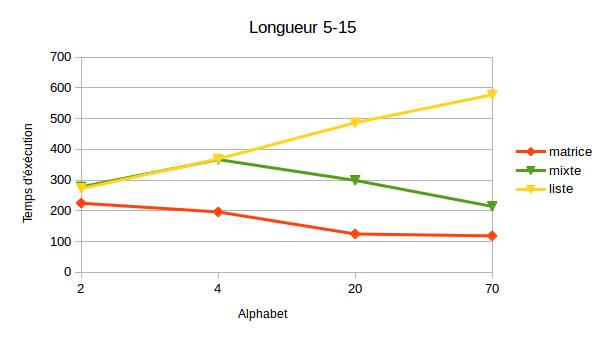
\includegraphics [width=30mm]{images/longueur5-15.jpg} \\[0.5cm]
  \begin{spacing}{1.5}
  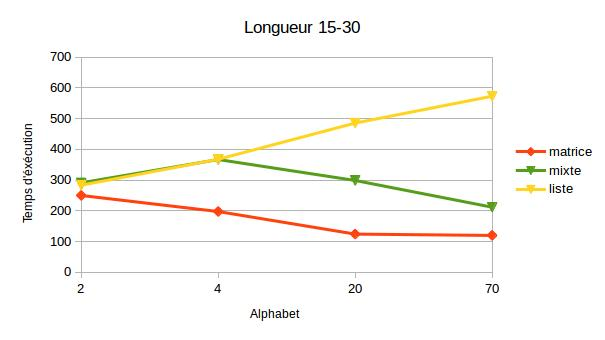
\includegraphics [width=30mm]{images/longueur15-30.jpg} \\[0.5cm]
  \begin{spacing}{1.5}
  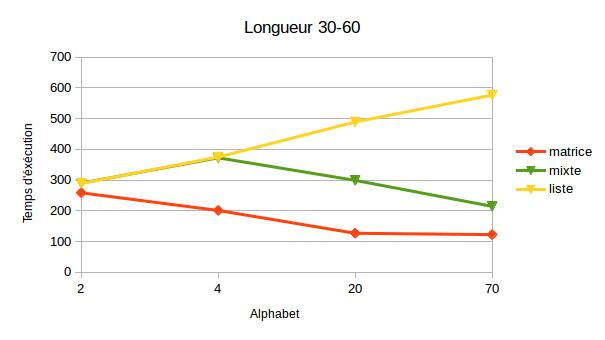
\includegraphics [width=30mm]{images/longueur30-60.jpg} \\[0.5cm]
  \begin{spacing}{1.5}
\subsubsection*{Conclusion sur les temps d'éxécution}
En analysant ces graphiques, on constate que la longueur des mots n'impliquent pas de changement majeur dans le temps d'éxécution.
De plus, les graphiques mettent en relief la différence de coût entre les différentes implémentations.
Nous voyons donc que dans tous les cas, le trie matriciel est plus rapide que le mixte
et le trie en liste.

\subsection{Taille dans la mémoire}
Afin d'obtenir la taille utilisée dans la mémoire pour chaque programme, nous avons
utilisé \emph{Valgrind}. Cet outil permet de corriger et de monitorer les variables
utilisées par un programme. Pour l'utiliser, nous avons exécuté la commande suivante :
\begin{minted}[gobble=4,framesep=5mm]{sh}
    valgrind --leak-check=full --show-leak-kinds=all
    --track-origins=yes PROGRAMME
\end{minted}
Avec \textbf{PROGRAMME} le nom du programme à vérifier. \emph{Valgrind} donne ensuite les fuites
de mémoires possible ainsi que le nombre d'octets pris dans la mémoire lors de
l'éxécution du programme.

\subsubsection*{Résultats sur la taille mémoire}

\begin{verbatim}
$ valgrind --leak-check=full --show-leak-kinds=all --track-origins=yes
bin/ac-matrice  gen/mots_a4_l5 gen/texte_a4
==4816== Memcheck, a memory error detector
==4816== Copyright (C) 2002-2013, and GNU GPL'd, by Julian Seward et al.
==4816== Using Valgrind-3.10.1 and LibVEX; rerun with -h for copyright info
==4816== Command: bin/ac-matrice gen/mots_a4_l5 gen/texte_a4
==4816==
[bin/ac-matrice] - count : 56730 (time : 2833ms)
==4816==
==4816== HEAP SUMMARY:
==4816==     in use at exit: 0 bytes in 0 blocks
==4816==   total heap usage: 765 allocs, 765 frees, 1,370,036 bytes allocated
==4816==
==4816== All heap blocks were freed -- no leaks are possible
==4816==
==4816== For counts of detected and suppressed errors, rerun with: -v
==4816== ERROR SUMMARY: 0 errors from 0 contexts (suppressed: 0 from 0)

$ valgrind --leak-check=full --show-leak-kinds=all --track-origins=yes
bin/ac-liste  gen/mots_a4_l5 gen/texte_a4
==4815== Memcheck, a memory error detector
==4815== Copyright (C) 2002-2013, and GNU GPL'd, by Julian Seward et al.
==4815== Using Valgrind-3.10.1 and LibVEX; rerun with -h for copyright info
==4815== Command: bin/ac-liste gen/mots_a4_l5 gen/texte_a4
==4815==
[bin/ac-liste] - count : 56730 (time : 7132ms)
==4815==
==4815== HEAP SUMMARY:
==4815==     in use at exit: 0 bytes in 0 blocks
==4815==   total heap usage: 1,514 allocs, 1,514 frees, 75,596 bytes allocated
==4815==
==4815== All heap blocks were freed -- no leaks are possible
==4815==
==4815== For counts of detected and suppressed errors, rerun with: -v
==4815== ERROR SUMMARY: 0 errors from 0 contexts (suppressed: 0 from 0)

$ valgrind --leak-check=full --show-leak-kinds=all --track-origins=yes
bin/ac-mixte  gen/mots_a4_l5 gen/texte_a4
==4817== Memcheck, a memory error detector
==4817== Copyright (C) 2002-2013, and GNU GPL'd, by Julian Seward et al.
==4817== Using Valgrind-3.10.1 and LibVEX; rerun with -h for copyright info
==4817== Command: bin/ac-mixte gen/mots_a4_l5 gen/texte_a4
==4817==
[bin/ac-mixte] - count : 56730 (time : 7206ms)
==4817==
==4817== HEAP SUMMARY:
==4817==     in use at exit: 0 bytes in 0 blocks
==4817==   total heap usage: 1,510 allocs, 1,510 frees, 77,524 bytes allocated
==4817==
==4817== All heap blocks were freed -- no leaks are possible
==4817==
==4817== For counts of detected and suppressed errors, rerun with: -v
==4817== ERROR SUMMARY: 0 errors from 0 contexts (suppressed: 0 from 0)
\end{verbatim}

Nous avons donc des complexités en espace, pour un fichier en entrée de \emph{5mo} :
\begin{itemize}
\item \textbf{Matrice} : 1370,036 ko
\item \textbf{Liste} : 75,596 ko
\item \textbf{Mixte} : 77,524 ko
\end{itemize}

\subsubsection*{Conclusion sur la taille mémoire}
Nous pouvons donc constater sur cet exemple, que le trie avec des matrices de
transitions prend environ \emph{17} fois plus de place que les deux autres, à cause de
ses nombreuses cases vides. Même si le trie prend relativement que peu de place
(\emph{1,3mo} sur un fichier de \emph{5mo}), s'il faut privilégier l'espace par rapport au temps,
le trie mixte ou en liste serait un bon choix.
